\documentclass[12pt, xcolor={svgnames,table}]{beamer}
%\documentclass[20pt,handout]{beamer}
\usetheme{Darmstadt}
\usepackage{graphicx}
%\usepackage[german]{babel}
\usepackage{ngerman}
\usepackage[T1]{fontenc}
\usepackage[utf8]{inputenc}
\usepackage{tikz}
\setbeamertemplate{footline}[frame number]

\newcommand{\cc}[1]{\includegraphics[height=4mm]{img/#1.png}\hspace{1mm}}
\usepackage{ifthen}
\newcommand{\license}[2][]{\\#2\ifthenelse{\equal{#1}{}}{}{\\\scriptsize\url{#1}}}
\usepackage{textcomp}
\usepackage{hyperref}

\pgfdeclareimage[height=.6cm]{c3d2logo}{./img/c3d2.pdf}


\pgfdeclarelayer{foreground}
\pgfsetlayers{main,foreground}
\logo{\pgfputat{\pgfxy(-1,0)}{\pgfbox[center,base]{\pgfuseimage{c3d2logo}}}}


\title{3 Jahre Snowden}
\author{\small Marius Melzer, Paul Schwanse\\\large Chaos Computer Club Dresden}
\date{23.03.2016}

\begin{document}
\maketitle

\section{Einleitung}
\subsection{}

\begin{frame}
    \frametitle{Chaos Computer Club}
    \begin{center}
	
\includegraphics[height=0.2\textheight]{img/chaosknoten.png}
    \end{center}	
    \begin{itemize}
      \item<1-> Verein wurde 1981 gegr"undet (\url{https://ccc.de})          
      \item<2-> Aktuell ca. 4500 Mitglieder
      \item<3-> Betreibt u.a. "Offentlichkeitsarbeit und Politikberatung      
    \end{itemize}
\end{frame}

\begin{frame}
  \frametitle{Chaos Computer Club}
  \begin{figure}
    
\includegraphics[height=0.7\textheight]{img/fingerabdruck.jpg}
  \end{figure}
\end{frame}

\begin{frame}
  \frametitle{Chaos Computer Club}
  \begin{figure}
    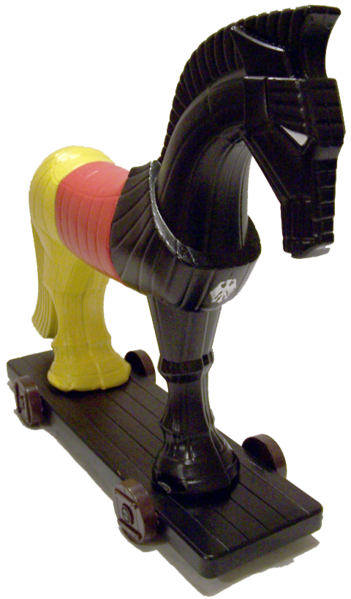
\includegraphics[height=0.7\textheight]{img/trojaner.png}
  \end{figure}
\end{frame}

\begin{frame}
    \frametitle{Chaos Computer Club}
    \begin{center}
	
\includegraphics[height=0.1\textheight]{img/c3d2_logo.png}
    \end{center}
    \begin{itemize}
      \item<1-> Chaos Computer Club Dresden (\url{https://c3d2.de})          
      \item<2-> Datenspuren (\url{https://datenspuren.de})
      \item<3-> Podcasts (\url{https://c3d2.de/radio.html})
      \item<4-> Chaos macht Schule (\url{https://c3d2.de/schule.html})
    \end{itemize}
\end{frame}

\section{Snowden Enthüllungen}
\subsection{}

\begin{frame}
    \frametitle{Bundespräsident Gauck zur NSA-Überwachung}
    \begin{center}
      ``Wir wissen z.B., dass es nicht so ist, wie bei der Stasi und dem KGB, dass es dicke Aktenbände gibt, wo unsere Gesprächsinhalte alle aufgeschrieben und schön abgeheftet sind. Das ist es nicht.''
      (Gauck, 30.06.2013 im ZDF-Sommerinterview)
    \end{center}
\end{frame}

\begin{frame}
    \frametitle{Stasi vs. NSA}
    \begin{center}
	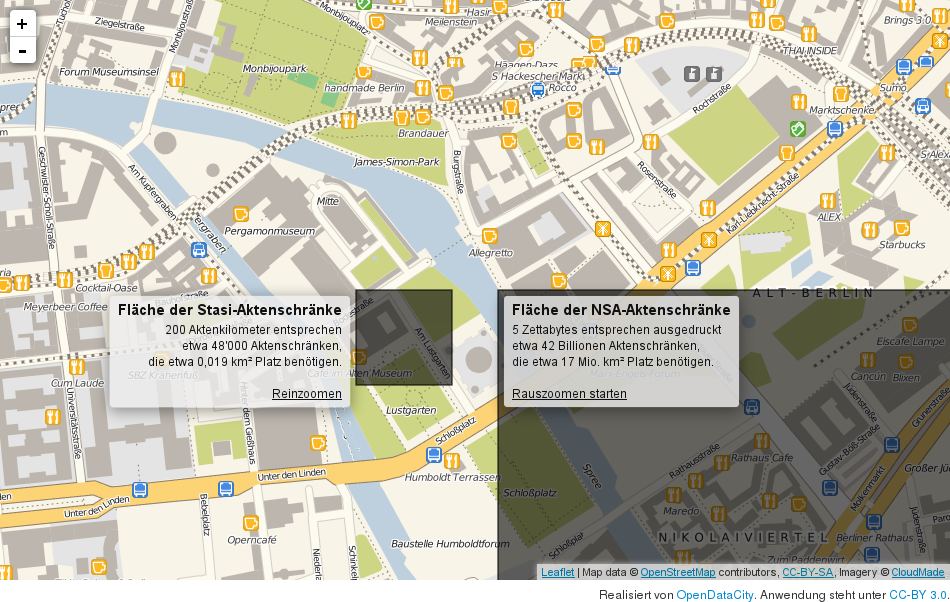
\includegraphics[height=0.7\textheight]{img/akten1.png}
    \end{center}
\end{frame}

\begin{frame}
    \frametitle{Stasi vs. NSA}
    \begin{center}
	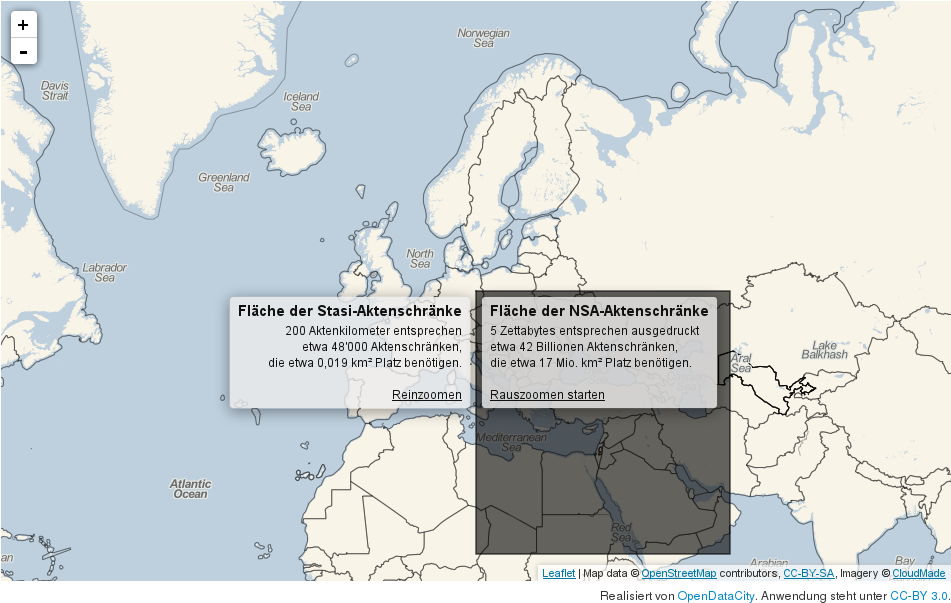
\includegraphics[height=0.7\textheight]{img/akten2.png}
    \end{center}
\end{frame}

\begin{frame}
    \frametitle{NSA-Skandal}
    \begin{center}
	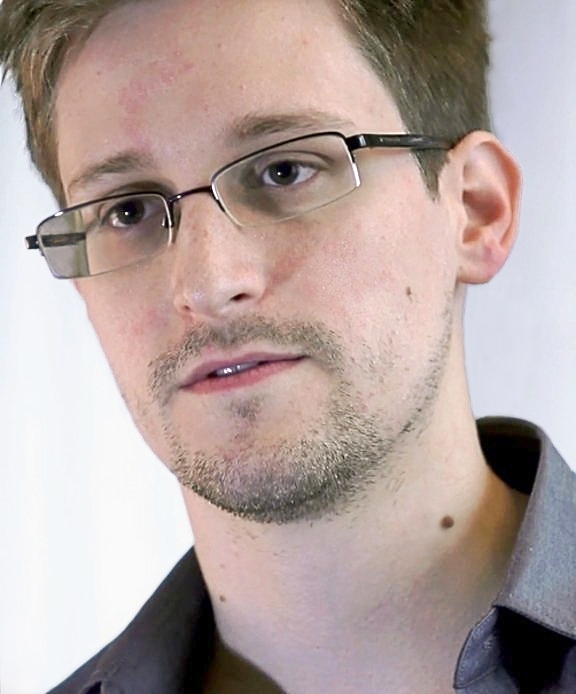
\includegraphics[height=0.7\textheight]{img/snowden.jpg}
	\\{\small \href{https://commons.wikimedia.org/wiki/File:Edward_Snowden.jpg\#mediaviewer/File:Edward_Snowden-2.jpg}{Grafik}: \href{https://creativecommons.org/licenses/by/3.0/}{\cc{by}} Laura Poitras / Praxis Films}
    \end{center}	
\end{frame}

% TODO Snowden Geschichte

\begin{frame}
  \frametitle{Tempora}
  \begin{center}
    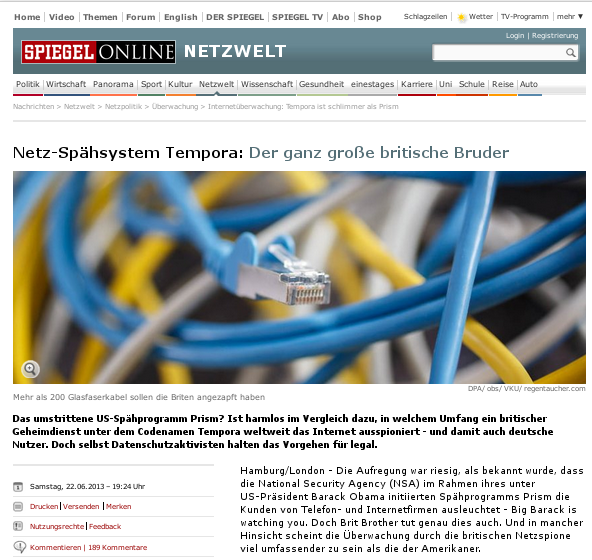
\includegraphics[height=0.7\textheight]{img/spiegel-tempora.png}
  \end{center}
\end{frame}

\begin{frame}
  \frametitle{Prism}
  \begin{center}
    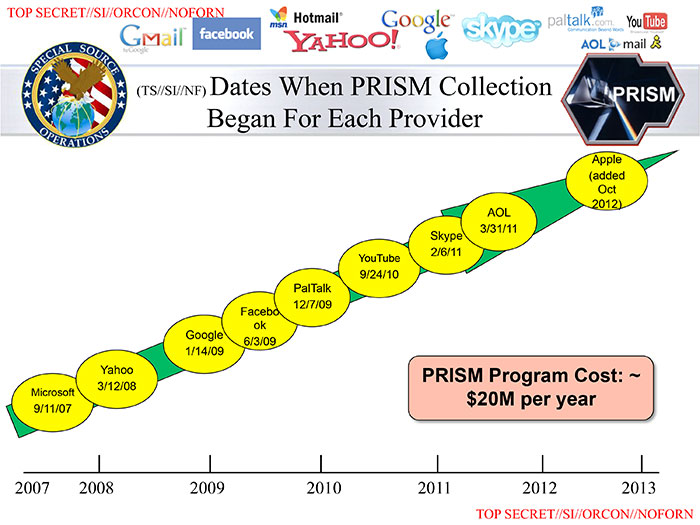
\includegraphics[height=0.7\textheight]{img/prism.jpg}
  \end{center}
\end{frame}

\begin{frame}
  \frametitle{Metadaten - Vorratsdatenspeicherung}
  \begin{center}
    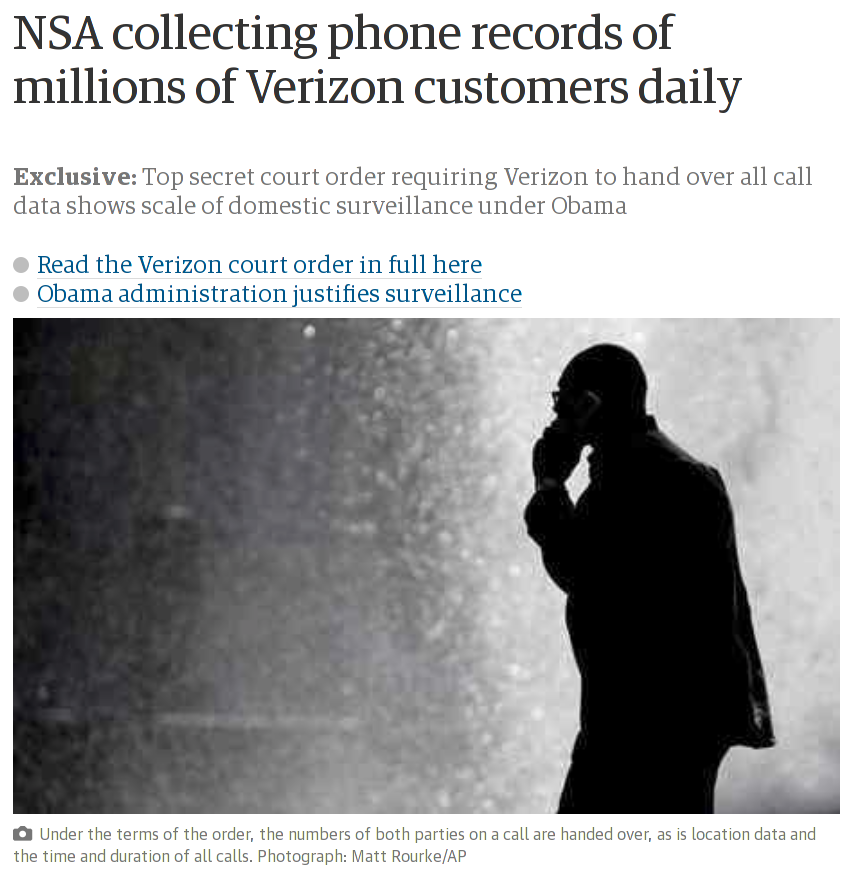
\includegraphics[height=0.7\textheight]{img/vds-verizon.png}
  \end{center}
\end{frame}

\begin{frame}
  \frametitle{Metadaten - Vorratsdatenspeicherung}
  \begin{itemize}
    \item Handynetz
      \begin{itemize}
        \item Telefonnummern
        \item Zeitpunkt und Dauer (Telefonate, SMS)
        \item Funkzelle (Ort)
      \end{itemize}
    \item Internet
      \begin{itemize}
        \item IP-Adresse (= ungefährer Ort)
        \item Alle Verbindungen
        \item Email: Adressen von Sender und Empfänger, Zugriff
      \end{itemize}
  \end{itemize}
\end{frame}

\begin{frame}
    \frametitle{Google Takeout}
    \begin{center}
      \includegraphics[width=0.8\textwidth]<1>{img/google_heat_1.png}
      \includegraphics[width=0.8\textwidth]<2>{img/google_heat_2.png}
    \end{center}
\end{frame}

\begin{frame}
    \frametitle{Zeitstempel}
    \begin{center}
      \only<1>{
        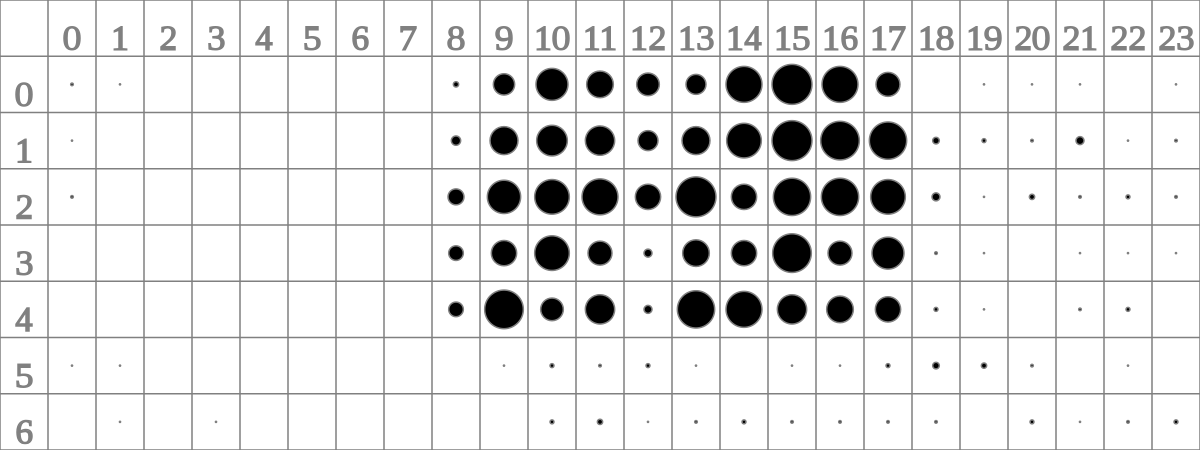
\includegraphics[width=0.9\textwidth]{img/punch_1.png}
        \\ \hfill \small Alan, Microblogging
      }

      \only<2>{
        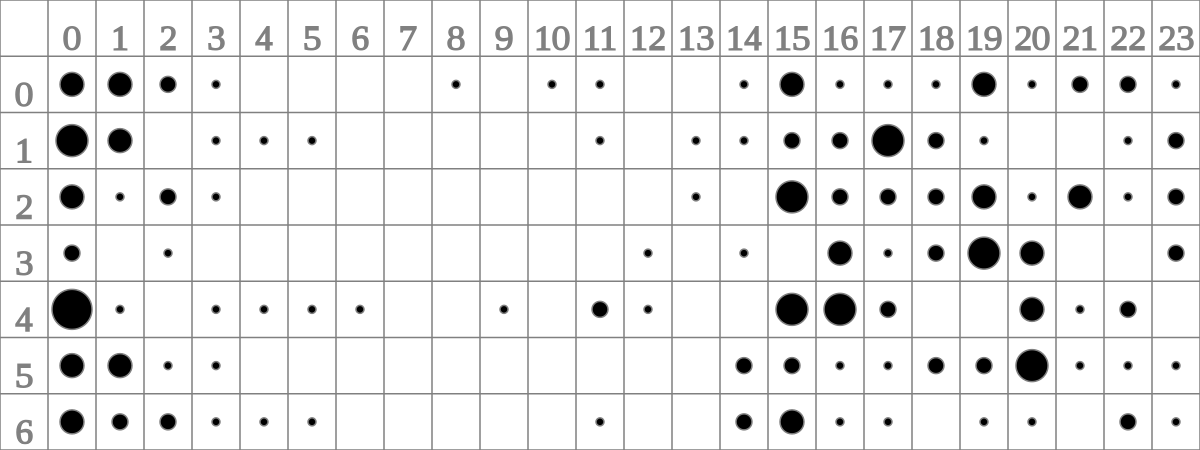
\includegraphics[width=0.9\textwidth]{img/punch_2.png}
        \\ \hfill \small Bob, Microblogging
      }

      \only<3>{
        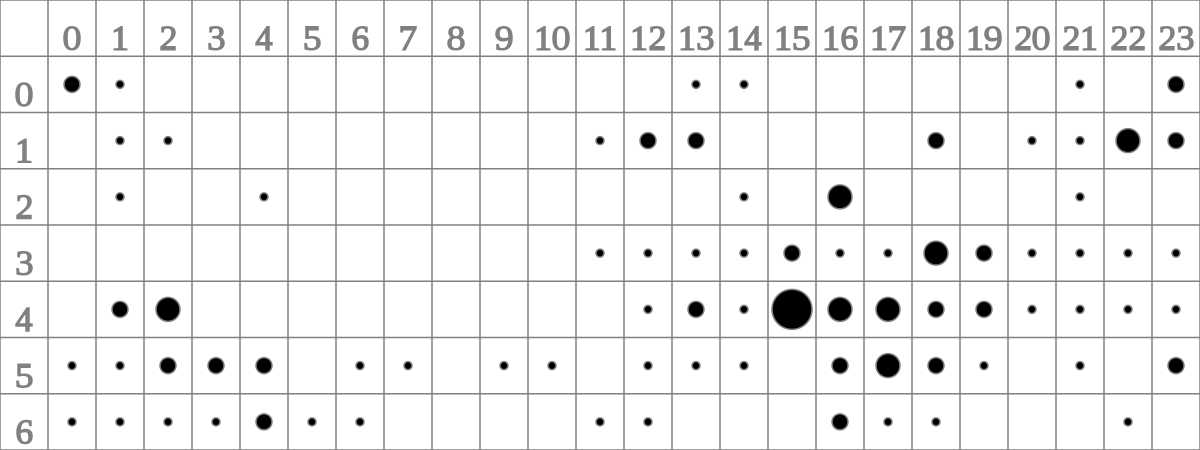
\includegraphics[width=0.9\textwidth]{img/punch_3.png}
        \\ \hfill \small Charlie, Github
      }
    \end{center}
\end{frame}

\begin{frame}
    \frametitle{Metadaten}
    \begin{center}
      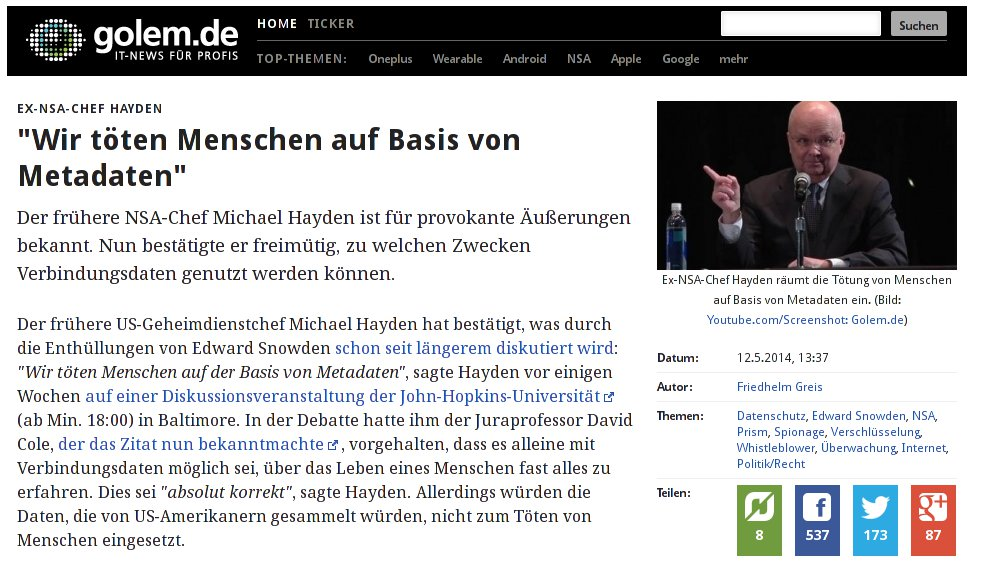
\includegraphics[height=0.7\textheight]{img/wekillpeople.jpg}
    \end{center}
\end{frame}

\section{Reaktionen}
\subsection{}

%TODO USA-Snowden - wie sind sie damit umgegangen (Landesverrat)? => Ministerpräsident von Chile, Greenwald-Partner

\begin{frame}
  \frametitle{Evo Morales}
    \begin{center}
      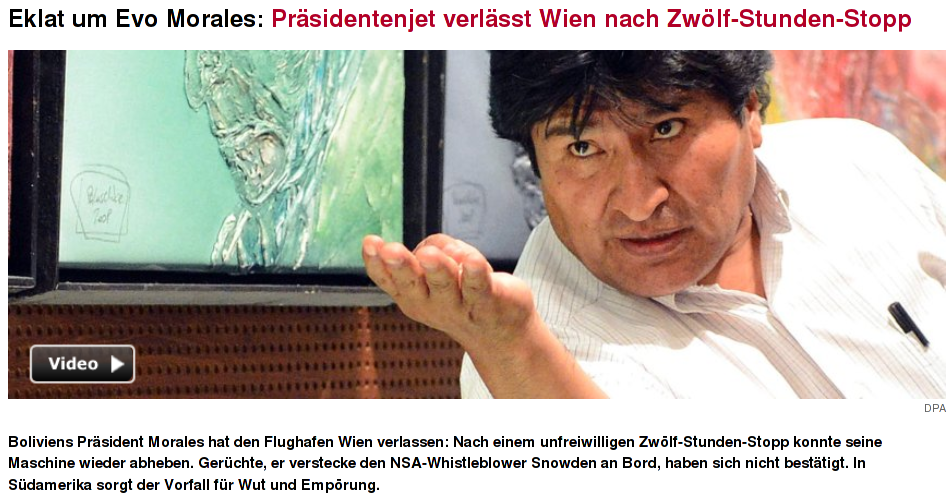
\includegraphics[height=5cm]{img/evomorales.png}
    \end{center}
\end{frame}

\begin{frame}
  \frametitle{Lavabit}
    \begin{center}
      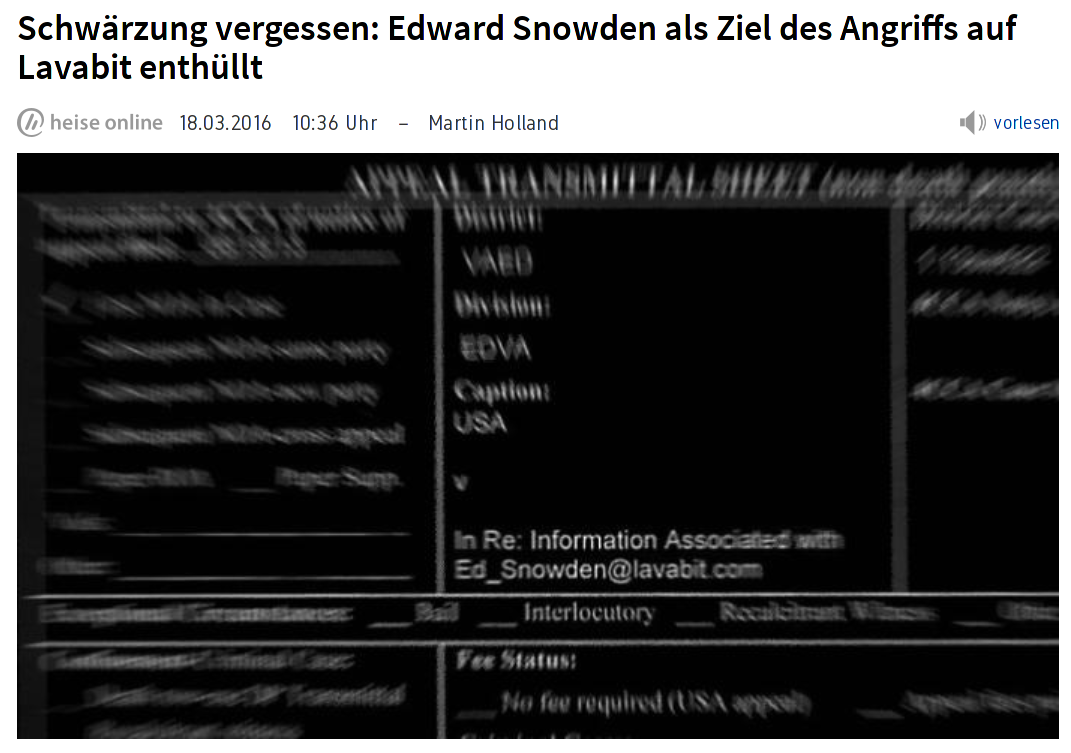
\includegraphics[height=5cm]{img/lavabit.png}
    \end{center}
\end{frame}

\begin{frame}
  \frametitle{Zusammenarbeit von NSA und Firmen}
    \begin{center}
      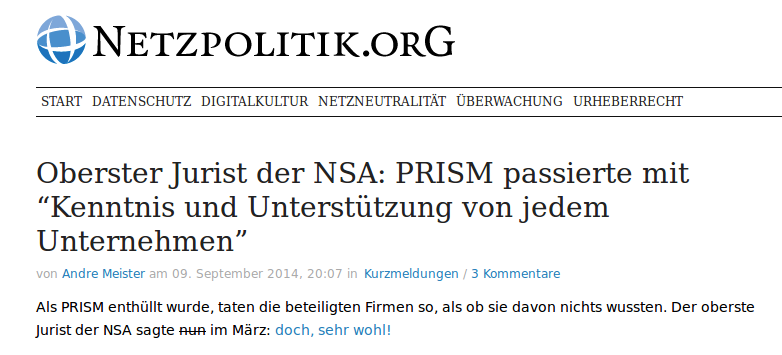
\includegraphics[height=5cm]{img/prism_netzpolitik.png}
    \end{center}
\end{frame}

\begin{frame}
    \frametitle{Datensparsamkeit?}
    \begin{center}
      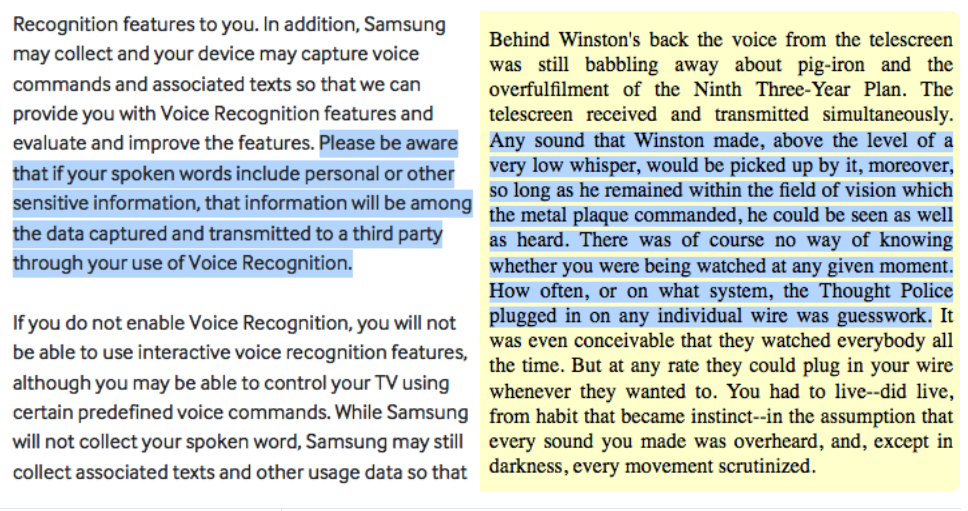
\includegraphics[height=0.7\textheight]{img/samsung-1984.png}
    \end{center}
\end{frame}

\begin{frame}
  \frametitle{Deutschland}
    \begin{center}
      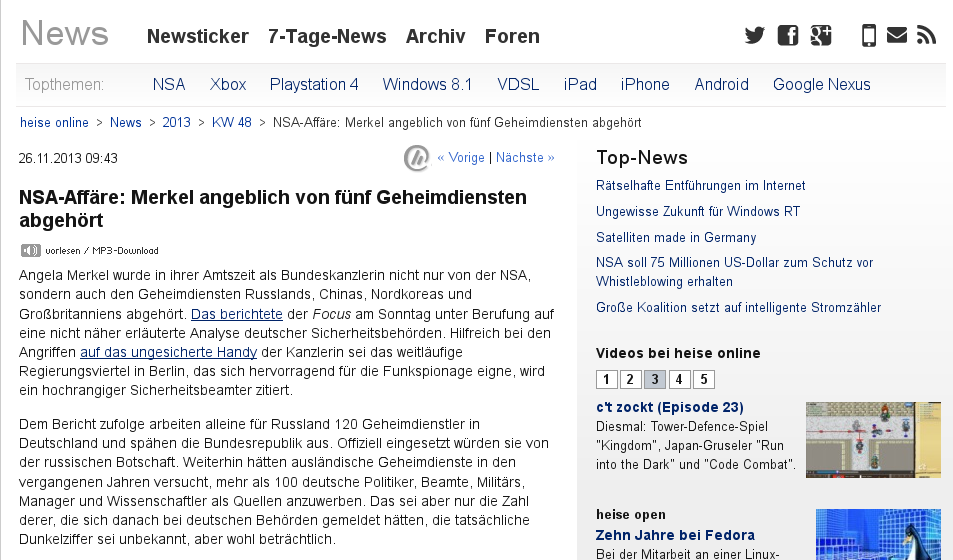
\includegraphics[height=5cm]{img/heise-merkel.png}
    \end{center}
\end{frame}

\begin{frame}
  \frametitle{NSAUA}
    \begin{center}
      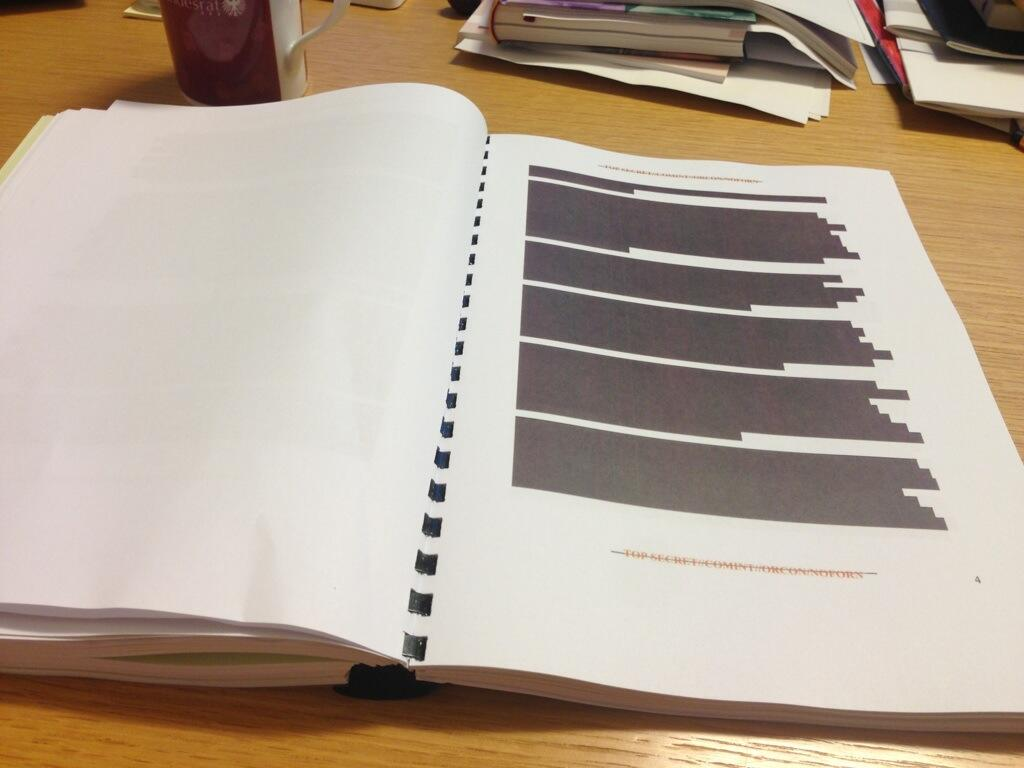
\includegraphics[height=5cm]{img/nsa-ua-akte.jpg}
    \end{center}
\end{frame}

\begin{frame}
  \frametitle{NSAUA Live-Blogs}
    \begin{center}
      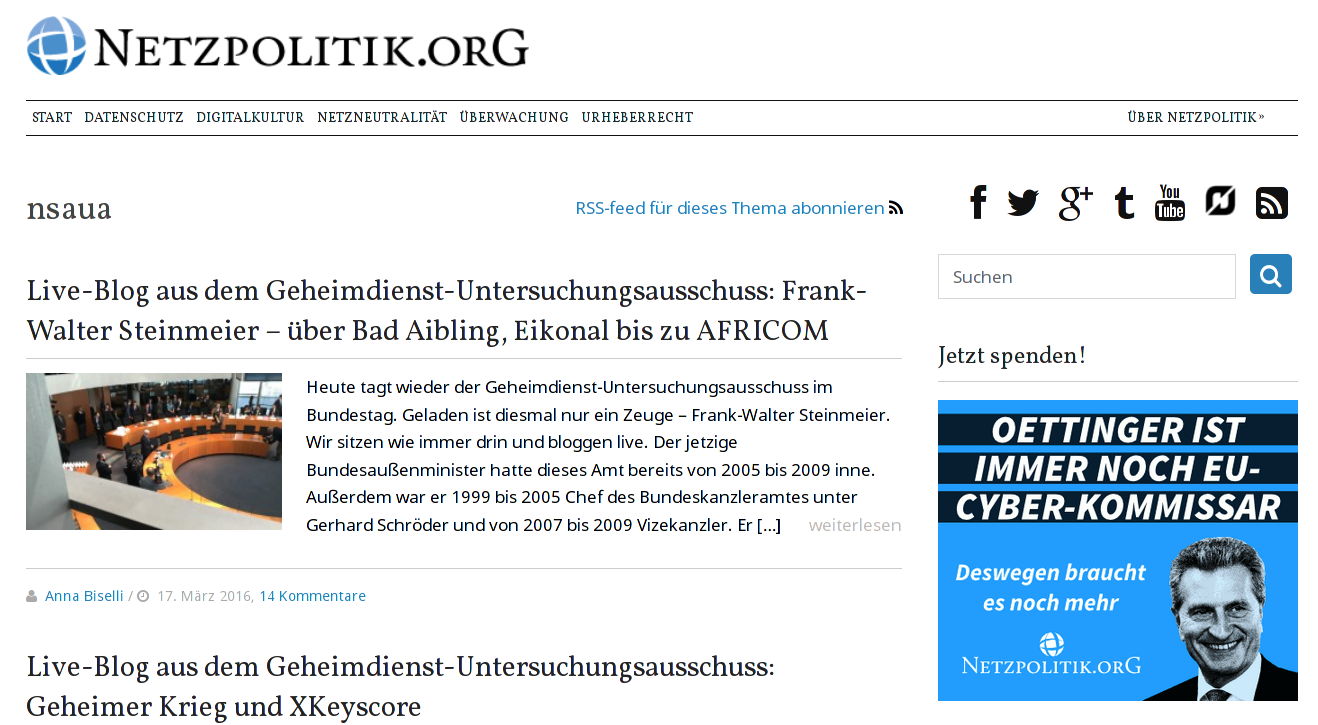
\includegraphics[height=5cm]{img/nsa-ua-netzpolitik.png}
    \end{center}
\end{frame}

\begin{frame}
  \frametitle{Selektorenaffäre}
    \small
    \begin{itemize}
      \item ~14 Millionen Selektoren von NSA durch BND angewandt
      \item 40.000 problematische Selektoren von BND aussortiert
      \item ``Sonderermittler'' Graulich: ~5.000 ``deutsche Grundrechtsträger'', ~22.000 staatliche Stellen (Dtl\&EU), ~1200 ``Verstöße gegen deutsche Interessen'' - spricht von ``klarem Vertragsbruch der NSA'', verteidigt BND und verschweigt Ausmaß und Betroffene
      \item Opposition aus NSAUA und G10-Kommission klagen vor dem Bundesverfassungsgericht
    \end{itemize}
\end{frame}

\begin{frame}
  \frametitle{Intelexit}
    \begin{center}
      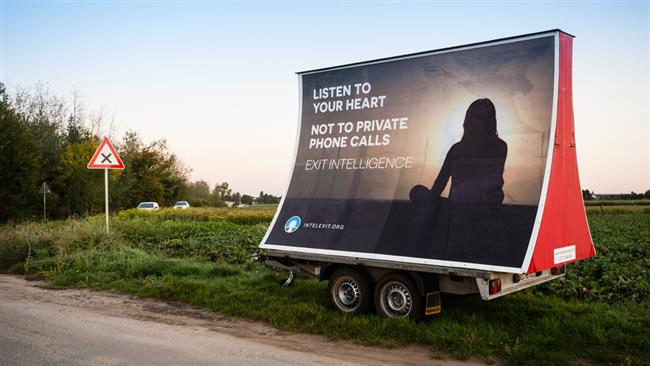
\includegraphics[height=5cm]{img/intelexit.jpg}
    \end{center}
\end{frame}

\section{Politische Entwicklungen}
\subsection{}

% TODO USA Freedom Act

\begin{frame}{EU-Datenschutzreform}
  \begin{columns}
    \column{5.5cm}
    \footnotesize

    \begin{itemize}
      \item Recht auf Vergessenwerden
      \item Datenportabilität
      \item Datensparsamkeit
      \item Informations- und Einwilligungspflicht
      \item Datenschutzfreundliche Voreinstellungen (Privacy by Design)
      \item gilt auch für Nicht-EU-Firmen, hohe Strafen (bis 4\% des Umsatzes) bei Verstößen
      \item kaum Erwähnung von neueren Phänomenen (Cloud, IoT,...)
    \end{itemize}

    \column{5cm}

    \begin{center}
      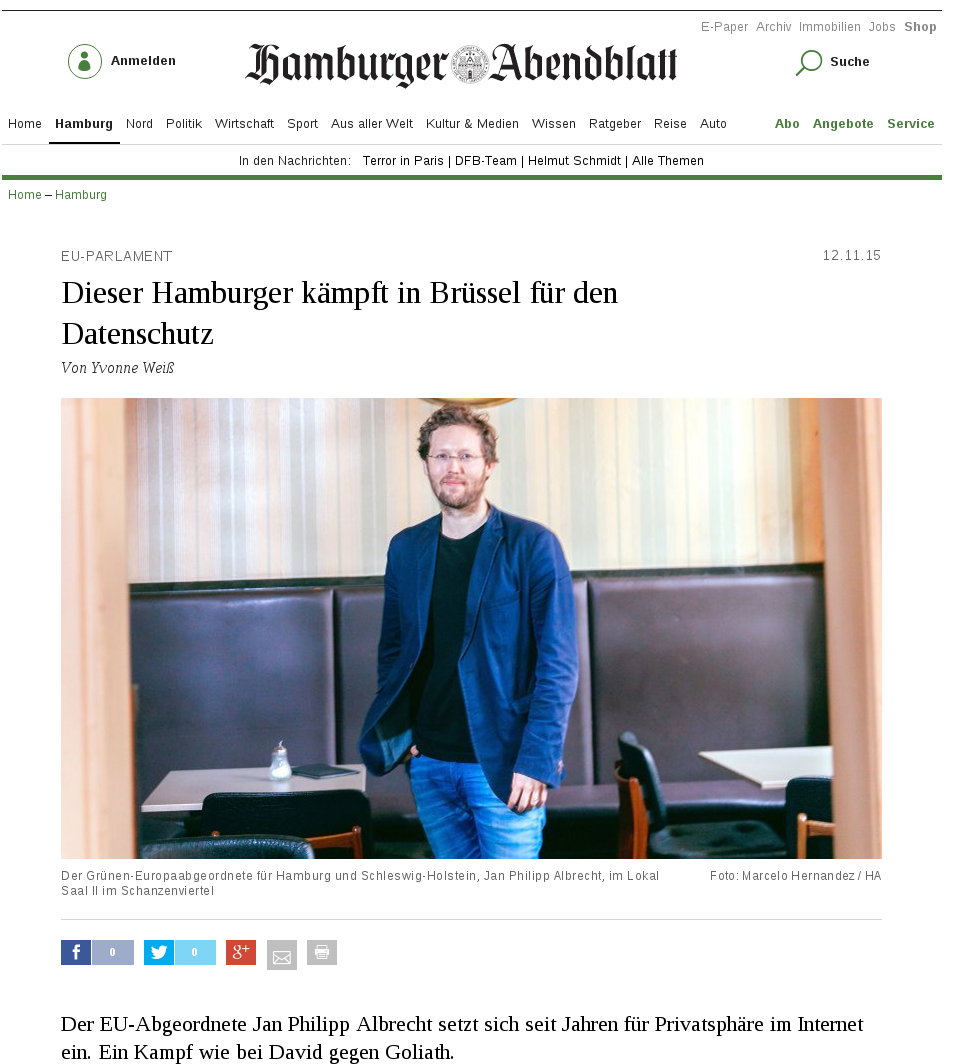
\includegraphics[width=4.5cm]{img/datenschutz-eu.png}
    \par\end{center}
  \end{columns}
\end{frame}

\begin{frame}
  \frametitle{Vorratsdatenspeicherung}
    \begin{center}
      \only<1>{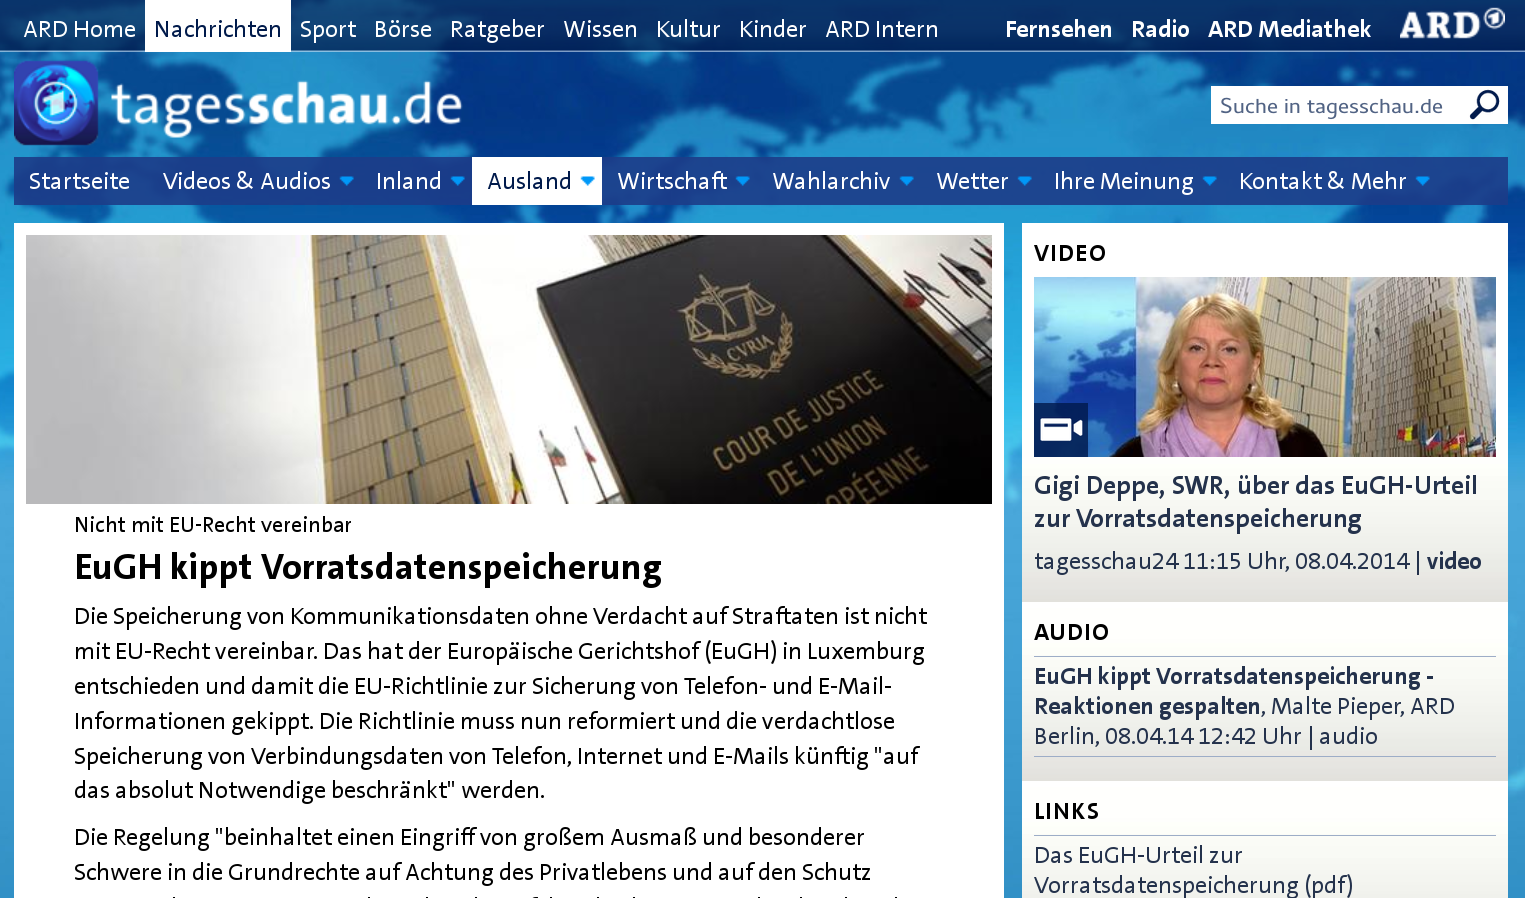
\includegraphics[height=5cm]{img/tagesschau-vds.png}}
      \only<2>{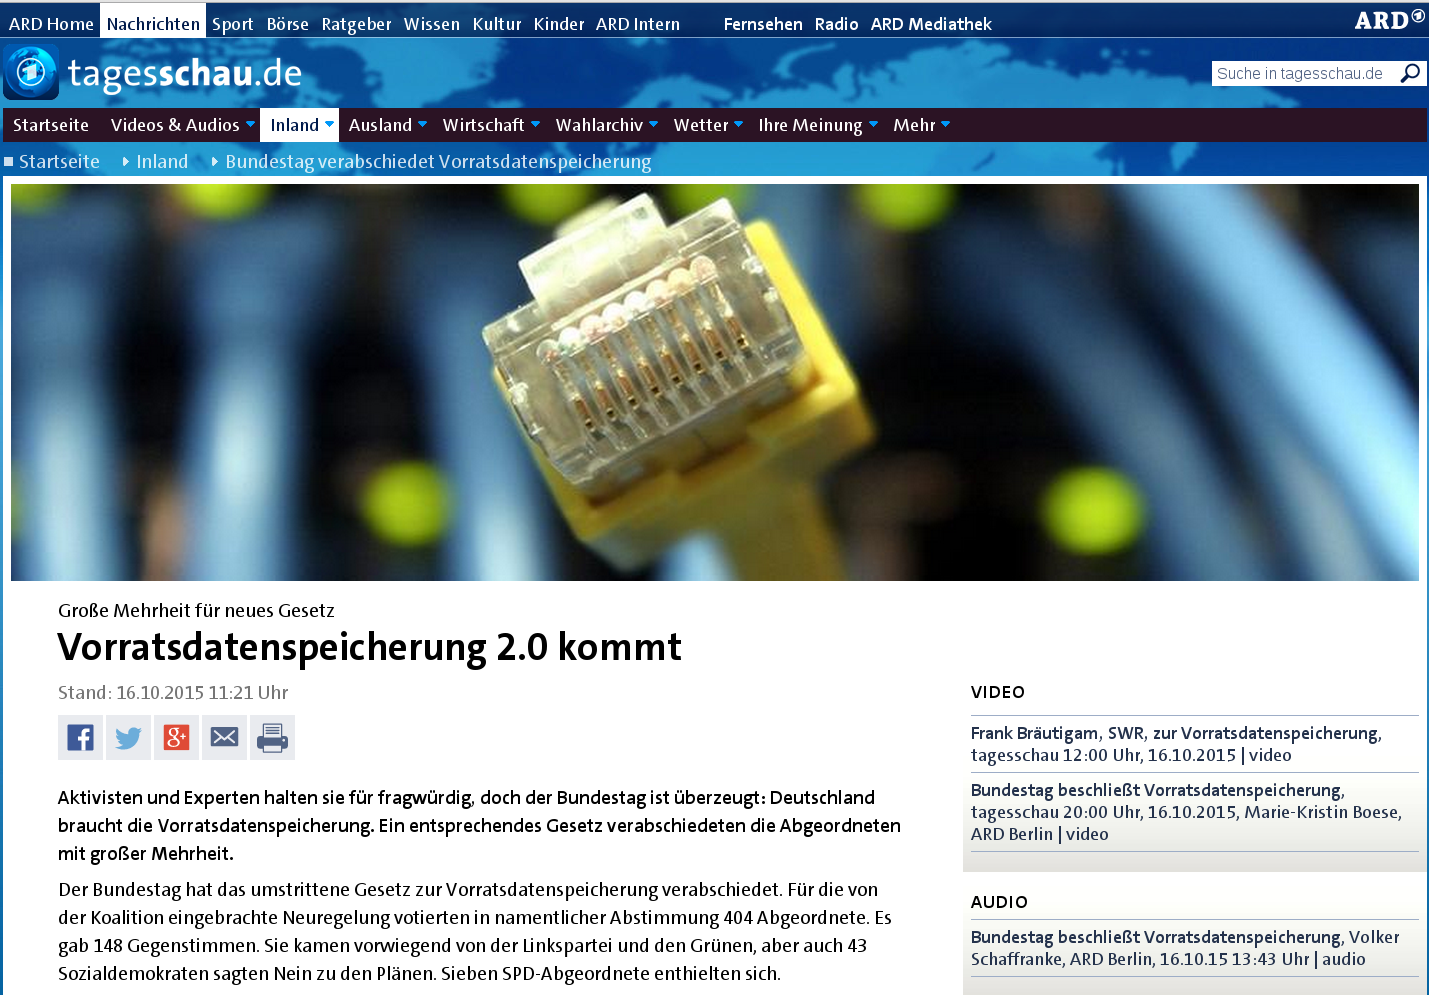
\includegraphics[height=5cm]{img/tagesschau-vds-2.png}}
    \end{center}
\end{frame}

% TODO Grund für Netzpolitik-Landesverrat

\begin{frame}
  \frametitle{Landesverrat}
  \begin{center}
    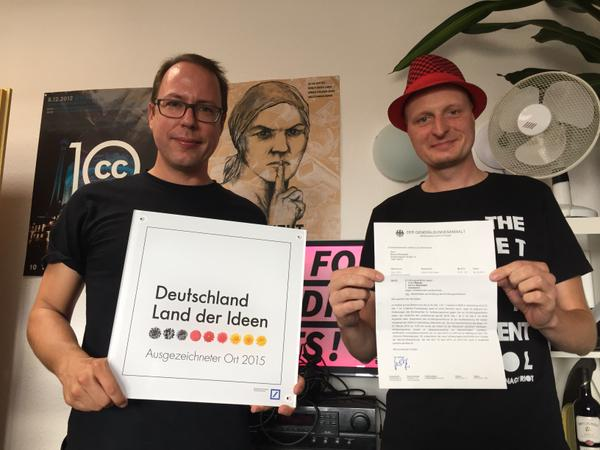
\includegraphics[height=0.7\textheight]{img/landesverrat.jpg}
  \end{center}
\end{frame}

\begin{frame}
  \frametitle{Safe Harbour}
  \begin{center}
    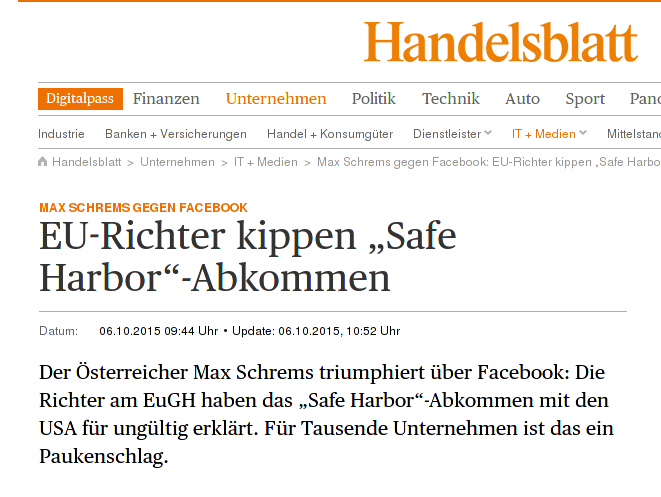
\includegraphics[height=0.7\textheight]{img/safeharbour.png}
  \end{center}
\end{frame}

% TODO Apple vs FBI
% TODO Facebook etc verschluesselung

\section{Technische Entwicklungen}
\subsection{}

\begin{frame}
  \frametitle{Vergleich Messenger}
  \small
  \begin{tabular}{|c|c|c|c|c|c|}
    \hline
                      & Whatsapp            & Threema             & Telegram              & Signal                & Jabber              \\
    \hline
    Verschlüsselung   & \cellcolor{orange}  & \cellcolor{yellow}  & \cellcolor{orange}    & \cellcolor{green}     & \cellcolor{green}   \\
    \hline
    Vertrauensw.      & \cellcolor{red}     & \cellcolor{yellow}  & \cellcolor{orange}    & \cellcolor{green}     & \cellcolor{green}   \\
    \hline
    Dezentr.          & \cellcolor{red}     & \cellcolor{red}     & \cellcolor{red}       & \cellcolor{orange}    & \cellcolor{green}   \\
    \hline
    Open Source       & \cellcolor{red}     & \cellcolor{red}     & \cellcolor{yellow}    & \cellcolor{green}     & \cellcolor{green}   \\
    \hline
    Mobileignung      & \cellcolor{green}   & \cellcolor{green}   & \cellcolor{green}     & \cellcolor{green}     & \cellcolor{yellow}  \\
    \hline
  \end{tabular}
\end{frame}

\begin{frame}
  \frametitle{Jabber: Conversations, ChatSecure}
    \begin{center}
      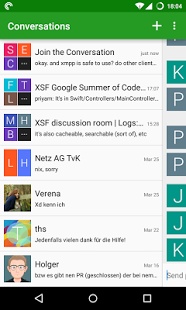
\includegraphics[height=5cm]{img/conversations.png}
      \hspace{0.5cm}
      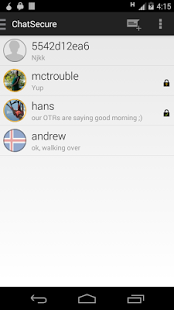
\includegraphics[height=5cm]{img/chatsecure.png}
    \end{center}
    \url{https://xmpp.net/directory.php}
\end{frame}

\begin{frame}
  \frametitle{Signal}
    \begin{center}
      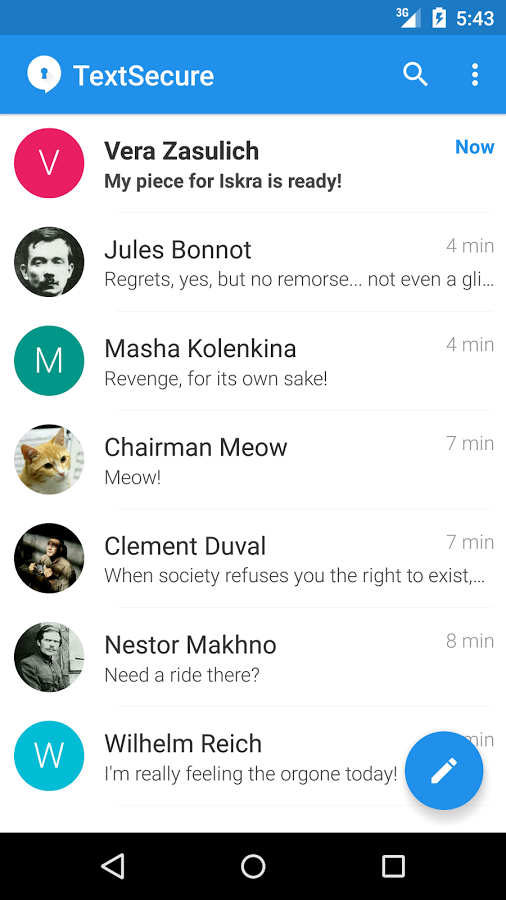
\includegraphics[height=6cm]{img/signal1.png}
      \hspace{0.5cm}
      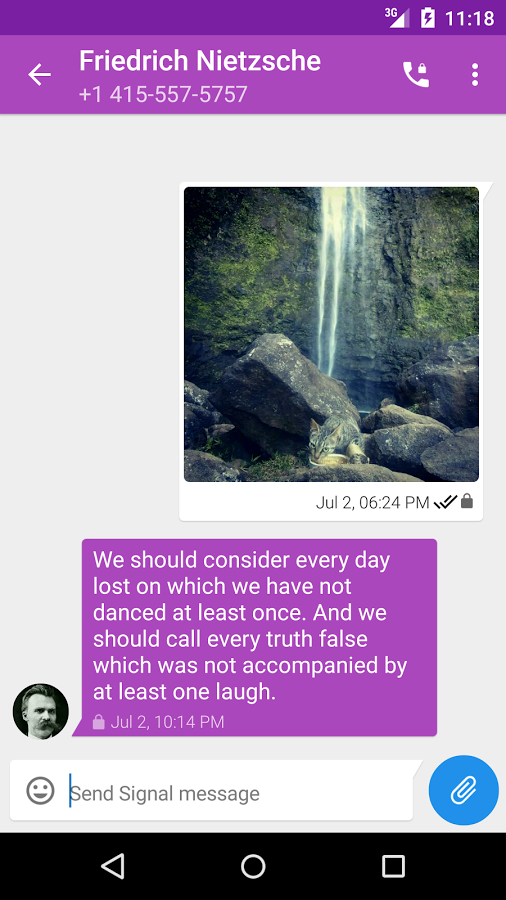
\includegraphics[height=6cm]{img/signal2.png}
    \end{center}
\end{frame}

\begin{frame}
  \frametitle{Snowden beim IETF}
    \begin{center}
      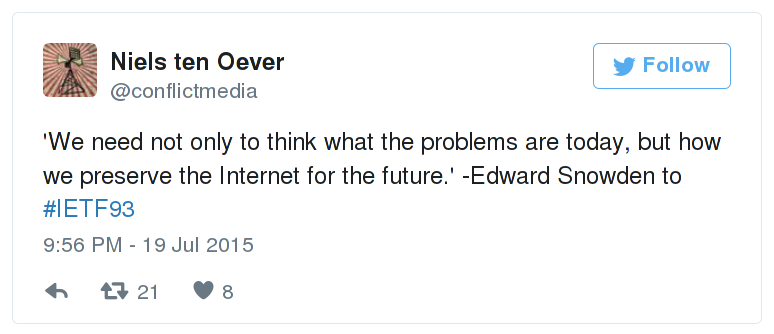
\includegraphics[height=4cm]{img/snowden-ietf.png}
    \end{center}
\end{frame}

\begin{frame}
  \frametitle{IETF vs. NSA}
    \begin{center}
      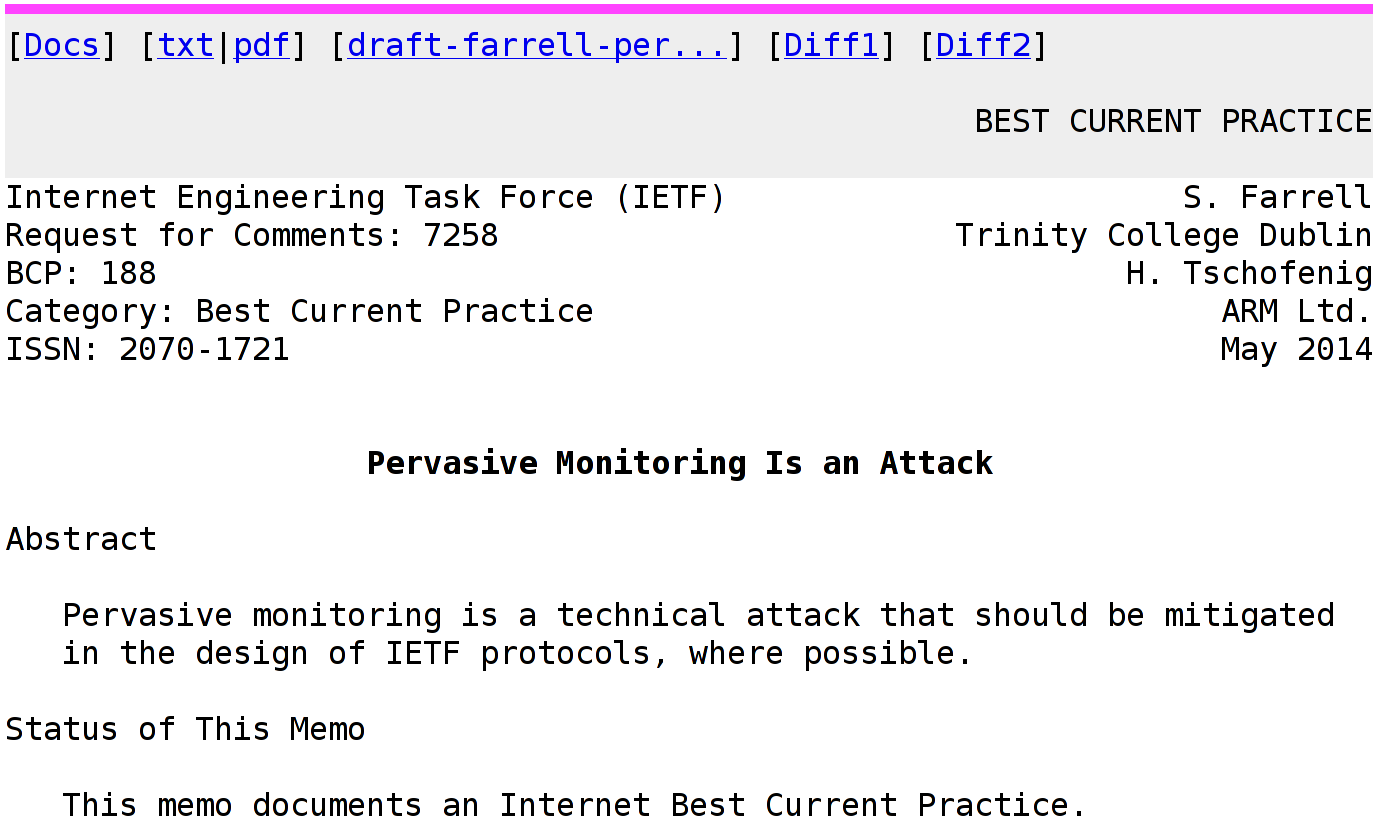
\includegraphics[height=5cm]{img/ietf-nsa.png}
    \end{center}
\end{frame}

\begin{frame}
  \frametitle{IETF vs. NSA}
    \footnotesize
    \begin{itemize}
      \item Verschlüsselung als Standard in künftigen Protokollen/-versionen
      \item Neue Nicht-NIST-elliptische Kurven (25519 von Bernstein, 448), benutzt in TLS, SSH, GPG
      \item MUST NOT: SSLv3, RC4, Schlüssellängen < 112 Bit
      \item SHOULD NOT: 3DES (Verschlüsselung), RSA (Schlüsselaustausch)
      \item MUST: Diffie-Hellmann, SHOULD: Schlüssellängen >= 2048
      \item TLS v1.0 und v1.1 nur wenn kein besserer Standard möglich
    \end{itemize}
\end{frame}

\begin{frame}
    \frametitle{Tor}
    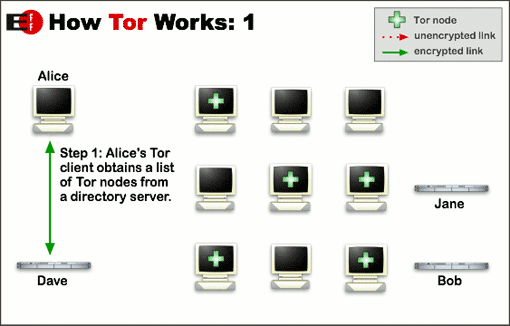
\includegraphics[height=0.7\textheight]{img/tor1.png}
    \\{\small \href{https://www.torproject.org/images/htw1.png}{Grafik}: \href{https://creativecommons.org/licenses/by/3.0/us/}{\cc{by}} The Tor Project}
\end{frame}

\begin{frame}
    \frametitle{Tor}
    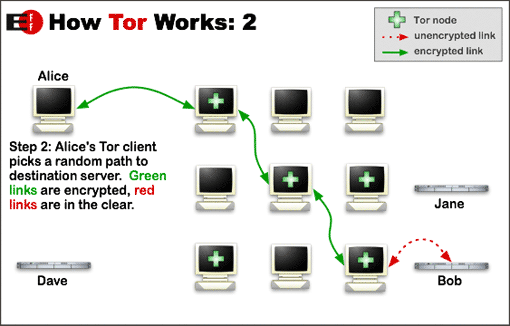
\includegraphics[height=0.7\textheight]{img/tor2.png}
    \\{\small \href{https://www.torproject.org/images/htw2.png}{Grafik}: \href{https://creativecommons.org/licenses/by/3.0/us/}{\cc{by}} The Tor Project}
\end{frame}

\begin{frame}
    \frametitle{Tor}
    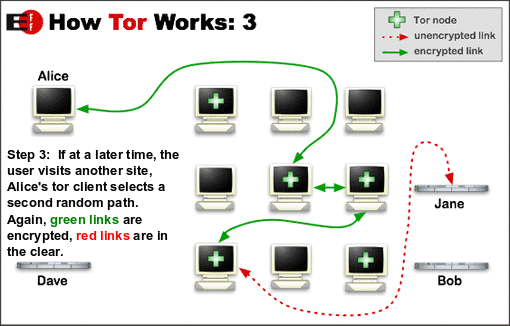
\includegraphics[height=0.7\textheight]{img/tor3.png}
    \\{\small \href{https://www.torproject.org/images/htw3.png}{Grafik}: \href{https://creativecommons.org/licenses/by/3.0/us/}{\cc{by}} The Tor Project}
\end{frame}

\begin{frame}{IETF und Tor}
  \begin{columns}
    \column{5.5cm}
    \footnotesize

    \begin{itemize}
      \item .onion als Spezialdomain anerkannt, darf nicht von der ICANN verteilt werden
      \item Könnte zukünftig Standarderweiterung für HTTP werden
    \end{itemize}

    \column{5cm}

    \begin{center}
      
\includegraphics[width=3.5cm]{img/tor-logo.jpg}
    \par\end{center}
  \end{columns}
\end{frame}

\begin{frame}{Facebook und Tor}
  \begin{columns}
    \column{5.5cm}
    \footnotesize

    \begin{itemize}
      \item Facebook nun auch als Onion Service erreichbar: https://facebookcorewwwi.onion/
      \item weltweit erstes TLS-Zertifikat für .onion Domain
    \end{itemize}

    \column{5cm}

    \begin{center}
      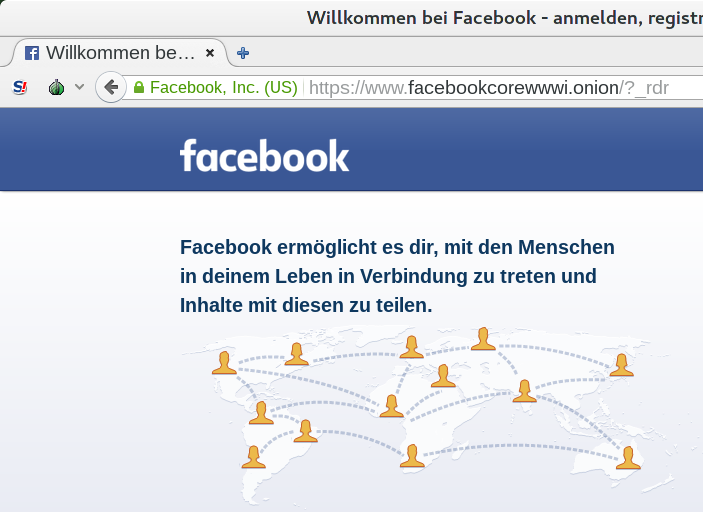
\includegraphics[width=4.5cm]{img/tor-facebook.png}
    \par\end{center}
  \end{columns}
\end{frame}

\begin{frame}{Let's encrypt}
  \begin{columns}
    \column{5.5cm}
    \footnotesize

    \begin{itemize}
      \item Certificate Authority für kostenlose und automatisierbar ausstellbare Zertifikate
      \item Definiertes Ziel allen Internetverkehr zu verschlüsseln
      \item schon in Beta fünftgrößte CA, seit Anfang März 1 Millionen ausgestellte Zertifikate
    \end{itemize}

    \column{5cm}

    \begin{center}
      
\includegraphics[width=3.5cm]{img/letsencrypt}
    \par\end{center}
  \end{columns}
\end{frame}

\section{Fazit}
\subsection{}

\begin{frame}
    \frametitle{Was sollten wir aus dem Snowden-Fall lernen?}
    \footnotesize
    \begin{itemize}
      \item Daten bedeuten Geld und Macht im ``Informationszeitalter''
      \item die eingeschlagenen politischen und technischen Wege bieten Raum für vorsichtigen Optimismus
      \item Wir brauchen einen Whistleblowerschutz und starke Gesetze für Datenschutz, Privacy by Design, Sicherheit von Infrastruktur (Abwesenheit von Backdoors)
      \item Änderung fängt beim Einzelnen an
    \end{itemize}
\end{frame}

\begin{frame}
    \frametitle{Technische Mittel zum Nachrecherchieren}
    \footnotesize
    \begin{itemize}
      \item Ende-zu-Ende-Verschlüsselung: PGP, Signal, Jabber mit OTR/OMEMO (Conversations, ChatSecure, Gajim),...
      \item Anonymisierung: Tor-Browser, Tor-Messenger, Ricochet
      \item Anti-Tracking: Disconnect, Privacy Badger, Ausschalten von Google AdID und Apple IDFA
      \item Verwendung von freier Software (Linux, CyanogenMod, F-Droid, etc.), Einschränken von Rechten (Permissions, Firewall)
    \end{itemize}
\end{frame}

\begin{frame}
    \frametitle{``Ich hab ja nichts zu vergergen''}
    \begin{center}
      ``Arguing that you don't care about the right to privacy because you have nothing to hide is no different than saying you don't care about free speech because you have nothing to say. ''
      (Edward Snowden, 21.05.2015 auf Reddit)
    \end{center}
\end{frame}

\begin{frame}
  \frametitle{Diskussion}
  \begin{center}
    {\Large Diskussion}\\
    \vspace{4mm}
    \href{https://github.com/c3d2/cms}{Folien}: \href{https://creativecommons.org/licenses/by-sa/4.0/}{\cc{by-sa}} Chaos Computer Club Dresden \\
    CMS Dresden: schule@c3d2.de\\
    \vspace{3mm}
    Vortragender: Marius Melzer (marius@rasumi.net, PGP-Fingerprint: 6730 E691 36B9 9BB8 FFB1 2662 A97B F176 52DE FC3E)
  \end{center}
\end{frame}

\end{document}
